% 20-minute proposal talk slides.
\documentclass[aspectratio=169,10pt]{beamer}

\usetheme{Boadilla}
\setbeamertemplate{navigation symbols}{}
\setbeamertemplate{footline}[frame number]

\usepackage{amsmath,amssymb}
\usepackage{booktabs}
\usepackage{xspace}
\usepackage{tikz}
\usetikzlibrary{arrows.meta,positioning,calc}

\definecolor{Dark}{HTML}{1D3557}
\definecolor{Accent}{HTML}{E07A5F}
\definecolor{Muted}{HTML}{6C757D}

\setbeamercolor{structure}{fg=Dark}
\setbeamercolor{frametitle}{fg=Dark}
\setbeamercolor{title}{fg=Dark}
\setbeamercolor{alerted text}{fg=Accent}

\newcommand{\hl}[1]{\textcolor{Accent}{#1}}
\newcommand{\muted}[1]{\textcolor{Muted}{#1}}

\newcommand{\SafetyIsland}{safety island\xspace}
\newcommand{\PrimaryCompute}{main CPU\xspace}
\newcommand{\FTTI}{FTTI\xspace}
\newcommand{\STL}{STL\xspace}

\title{Cache-Coherent Safety Islands for Low-Latency CPS Policy Monitoring}
\subtitle{Project proposal: intent export + runtime policy checks within an \FTTI budget}
\author{Nazmus Shakib Sayom}
\institute{University of Utah}
\date{February 2026}

\begin{document}

\begin{frame}
  \titlepage
\end{frame}

\begin{frame}{Motivation: Functional Safety Implies Bounded Time}
\begin{itemize}
\item Functional safety requires detecting and controlling faults before hazards occur.
\item The fault-tolerant time interval (\FTTI) bounds how long we can take to \emph{detect + react}.
\item Modern CPS/automotive SoCs already include a \SafetyIsland: isolated compute that can supervise the main system and force a fail-safe reaction.
\end{itemize}

\vspace{0.8em}
\textbf{Opportunity:} Move beyond watchdogs and fault flags to \hl{online policy monitoring} over real signals.
\end{frame}

\begin{frame}{Safety Islands: Where They Sit and What They Do}
\begin{itemize}
\item \textbf{Isolation.} Separate core(s), memory region, and trusted software stack.
\item \textbf{Supervision.} Observe system health and safety-relevant signals; decide when to trigger a safe state.
\item \textbf{Interfaces.} Today, many interfaces are coarse (fault flags, watchdog kicks, periodic status).
\end{itemize}

\vspace{0.8em}
\textbf{Gap for this project:} architecture support to let the \SafetyIsland check \emph{behavioral safety policies} fast enough to matter.
\end{frame}

\begin{frame}{Policy Monitoring: Intent vs.\ Evidence}
\textbf{Idea.} Check that the system's behavior stays within a safety envelope over time (deadlines, dwell times, tolerances).

\vspace{0.6em}
\begin{itemize}
\item We need two views:
  \begin{itemize}
  \item \hl{Intent}: what the controller asked for.
  \item \hl{Evidence}: what the system actually did.
  \end{itemize}
\item The \SafetyIsland correlates them and triggers a reaction if the policy is violated.
\end{itemize}
\end{frame}

\begin{frame}{Example: PWM Actuation Integrity (Stress Test)}
\begin{center}
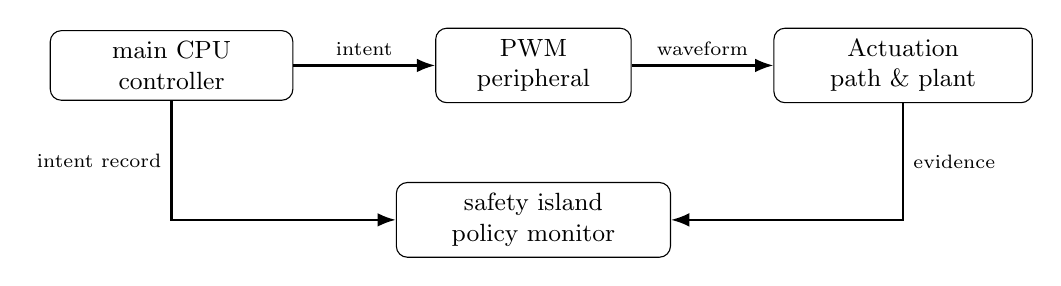
\begin{tikzpicture}[
    box/.style={draw,rounded corners,align=center,inner sep=4pt,font=\small},
    arr/.style={-Latex,thick},
    node distance=8mm and 18mm,
  ]
  \node[box, text width=2.8cm] (ctrl) {\PrimaryCompute\\controller};
  \node[box, right=of ctrl, text width=2.2cm] (pwm) {PWM\\peripheral};
  \node[box, right=of pwm, text width=3.0cm] (plant) {Actuation\\path \& plant};

  \draw[arr] (ctrl) -- node[above, font=\scriptsize]{intent} (pwm);
  \draw[arr] (pwm) -- node[above, font=\scriptsize]{waveform} (plant);

  \node[box, below=of pwm, yshift=-2mm, text width=3.2cm] (si) {\SafetyIsland\\policy monitor};
  \draw[arr] (ctrl.south) |- node[pos=0.25, left, font=\scriptsize]{intent record} (si.west);
  \draw[arr] (plant.south) |- node[pos=0.25, right, font=\scriptsize]{evidence} (si.east);
\end{tikzpicture}
\end{center}

\begin{itemize}
\item Even correct control software can be undermined by faults/timing interference downstream.
\item We need policies that relate \emph{intended} and \emph{realized} actuation with deadlines/dwell times.
\end{itemize}
\end{frame}

\begin{frame}{Problem Statement}
\textbf{We want:} check safety policies within \FTTI, using intent and evidence that live in different protection domains.

\vspace{0.6em}
\textbf{Constraints.}
\begin{itemize}
\item \textbf{Low latency:} the monitor must see new controller intent quickly.
\item \textbf{Low overhead:} intent export should not burden the control loop.
\item \textbf{Correctness:} the island must read a \emph{consistent} controller record (not a mixed snapshot).
\item \textbf{Predictability:} worst-case export + monitoring time must be bounded under contention.
\end{itemize}
\end{frame}

\begin{frame}{Goal and Hypothesis (Once the Context Is Set)}
\textbf{Hypothesis.} \hl{Cache-coherent shared memory} is the best substrate for low-latency intent export from the \PrimaryCompute to an MCU-like \SafetyIsland monitor.

\vspace{0.6em}
\textbf{Project goal.} Define the \hl{architecture contract} that makes coherent monitoring both correct and time-bounded:
\begin{itemize}
\item coherent interface choice for an MCU-like \SafetyIsland,
\item synchronization discipline for multi-field records,
\item predictability mechanisms to meet \FTTI.
\end{itemize}
\end{frame}

\begin{frame}{Why Cache-Coherent Shared Memory? (Pro-Coherence)}
\textbf{Goal:} export controller intent to the \SafetyIsland with \hl{minimal latency and overhead}.

\vspace{0.4em}
\begin{itemize}
\item \textbf{Single-copy path:} controller writes once; island reads via ordinary loads (no message copying).
\item \textbf{Fast steady state:} avoids software-managed cache maintenance and explicit DMA staging.
\item \textbf{Good fit for control:} frequent small records, tight deadlines.
\end{itemize}

\vspace{0.7em}
\textbf{One-sentence definition.} Cache coherence keeps caches consistent so both cores observe a single up-to-date value \emph{per memory location}.

\vspace{0.4em}
\textbf{Important nuance.} The project is to design the missing pieces for \emph{snapshot correctness} and \emph{bounded latency}.
\end{frame}

\begin{frame}{Proposed Architecture (High Level)}
\begin{center}
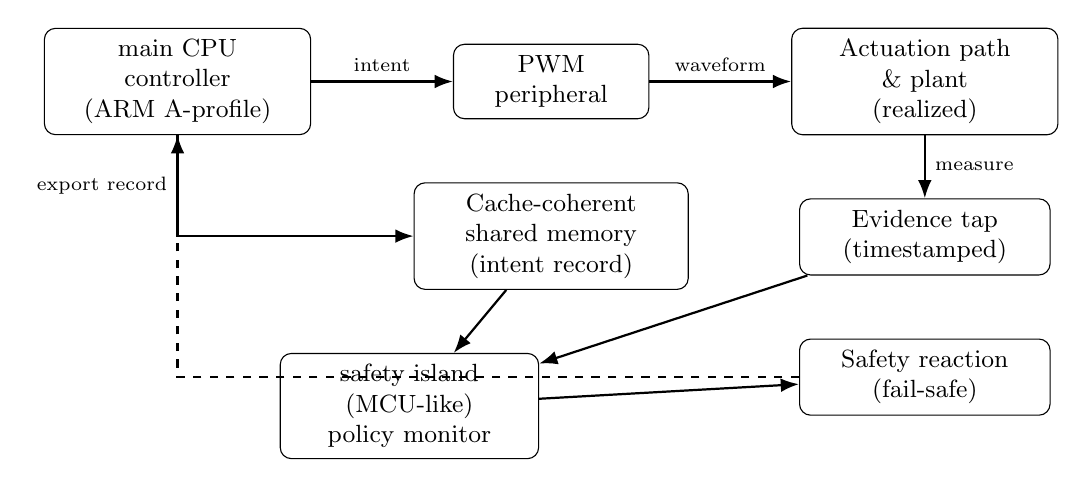
\begin{tikzpicture}[
    box/.style={draw,rounded corners,align=center,inner sep=4pt,font=\small},
    arr/.style={-Latex,thick},
    node distance=8mm and 18mm,
  ]
  \node[box, text width=3.1cm] (ctrl) {\PrimaryCompute\\controller\\(ARM A-profile)};
  \node[box, right=of ctrl, text width=2.2cm] (pwm) {PWM\\peripheral};
  \node[box, right=of pwm, text width=3.1cm] (plant) {Actuation path\\\& plant\\(realized)};

  \node[box, below=of pwm, text width=3.2cm] (shm) {Cache-coherent\\shared memory\\(intent record)};
  \node[box, below=of plant, text width=2.9cm] (evidence) {Evidence tap\\(timestamped)};

  \node[box, below=of shm, xshift=-18mm, text width=3.0cm] (si) {\SafetyIsland\\(MCU-like)\\policy monitor};
  \node[box, below=of evidence, text width=2.9cm] (react) {Safety reaction\\(fail-safe)};

  \draw[arr] (ctrl) -- node[above, font=\scriptsize]{intent} (pwm);
  \draw[arr] (pwm) -- node[above, font=\scriptsize]{waveform} (plant);
  \draw[arr] (ctrl.south) |- node[pos=0.25, left, font=\scriptsize]{export record} (shm.west);
  \draw[arr] (plant.south) -- node[right, font=\scriptsize]{measure} (evidence.north);
  \draw[arr] (shm) -- (si);
  \draw[arr] (evidence) -- (si);
  \draw[arr] (si) -- (react);
  \draw[arr,dashed] (react.west) -| (ctrl.south);
\end{tikzpicture}
\end{center}

\vspace{-0.2em}
\muted{Key idea:} coherence gives a low-latency export path; we design the interface contract that makes it reliable under weak ordering and contention.
\end{frame}

\begin{frame}{Challenge: Reading a Consistent Record}
\textbf{Weak ordering:} other cores may observe your writes in a different order than your program order (unless you synchronize).

\vspace{0.6em}
\begin{columns}[T,onlytextwidth]
  \column{0.52\textwidth}
  \textbf{Writer (controller)}
  \begin{itemize}
  \item store duty := new
  \item store ts := new
  \end{itemize}

  \column{0.48\textwidth}
  \textbf{Reader (\SafetyIsland)}
  \begin{itemize}
  \item load ts == new
  \item load duty == old \alert{(mixed step)}
  \end{itemize}
\end{columns}

\vspace{0.8em}
\textbf{Design task:} define an \hl{export record + synchronization discipline} so island reads behave like consistent ``steps.''
\end{frame}

\begin{frame}{Challenge: Worst-Case Latency Under Contention}
\begin{itemize}
\item Coherence implies traffic (line transfers, invalidations/snoops, directory activity).
\item Shared caches and interconnect arbitration add variability.
\item Worst-case export+monitor latency must satisfy: \[
  \Delta_{\text{export}} + \Delta_{\text{monitor}} + \Delta_{\text{react}} \le \FTTI.
\]
\end{itemize}

\vspace{0.8em}
\textbf{Design task:} identify \hl{predictability mechanisms} (partitioning, priorities, protocol choices) that bound worst-case coherent-access latency.
\end{frame}

\begin{frame}{Prior Work: What We Build On (and What's Missing)}
\begin{itemize}
\item \textbf{Safety islands exist:} strong isolation and supervisory logic are well established.
\item \textbf{Runtime verification exists:} temporal-policy monitoring is mature, including robustness ideas for noisy signals.
\item \textbf{Real-time coherence exists:} there is prior work on making coherent memory systems more predictable.
\end{itemize}

\vspace{0.8em}
\textbf{Gap (this project).} An application-driven \hl{contract} that connects these: a cache-coherent safety-island architecture for policy monitoring within \FTTI, with explicit snapshot correctness, time alignment, and worst-case latency bounds.
\end{frame}

\begin{frame}{Research Questions}
\begin{itemize}
\item \textbf{RQ1 (Coherent interface).} How should an MCU-like \SafetyIsland participate in coherence with an A-profile \PrimaryCompute?
\item \textbf{RQ2 (Snapshot correctness).} What record format + synchronization rules guarantee consistent multi-field snapshots under weak ordering?
\item \textbf{RQ3 (Predictability).} What worst-case export and monitoring latency bounds are achievable under contention, and what mechanisms enforce them?
\item \textbf{RQ4 (Evidence and time alignment).} Where do we measure realized actuation, and how do we align evidence with controller records?
\end{itemize}
\end{frame}

\begin{frame}{Policy Monitoring Model (STL as a Representative Choice)}
\begin{itemize}
\item Policies are temporal constraints over signals (deadlines, dwell times, envelopes).
\item \STL is one common language; the architecture should support other temporal formalisms too.
\item Robust monitoring outputs a \textbf{margin} (how close to violation), useful under noise.
\end{itemize}

\vspace{0.6em}
\textbf{Monitor I/O.}
\begin{itemize}
\item Inputs: controller record stream + evidence stream (time-aligned).
\item Output: violation / negative robustness $\Rightarrow$ trigger safety reaction.
\end{itemize}
\end{frame}

\begin{frame}{Case Study: PWM Actuation Integrity}
\textbf{Signals.}
\begin{itemize}
\item Intent (from shared record): duty, dead-time, update sequence, timestamp.
\item Evidence: edge timings / waveform-derived duty, glitch signatures, timing anomalies.
\end{itemize}

\vspace{0.6em}
\textbf{Example policies (illustrative).}
\begin{itemize}
\item Tracking: realized duty converges to intended duty within a deadline and stays within tolerance.
\item Glitch exclusion: no pulses below a minimum width.
\item Safety envelope: upon a safety condition, realized PWM enters a conservative envelope within a deadline.
\end{itemize}
\end{frame}

\begin{frame}{Soundness Story (Conditional)}
\textbf{Claim shape.} Under explicit interface + timing assumptions, the \SafetyIsland monitor's decision matches the intended policy semantics \emph{in time} to react within \FTTI.

\vspace{0.6em}
\textbf{Key assumptions we will make explicit and validate:}
\begin{itemize}
\item Coherent export path with a synchronization discipline that yields consistent snapshots.
\item Bounded skew between controller timestamps and evidence timestamps.
\item Worst-case export+monitor+reaction latency within \FTTI.
\end{itemize}
\end{frame}

\begin{frame}{Evaluation Plan (What We Will Measure/Show)}
\begin{itemize}
\item \textbf{Snapshot failure modes:} demonstrate how naive coherent sharing yields mixed records; show the minimal synchronization contract that fixes it.
\item \textbf{Latency under contention:} microbench coherent export latency with controlled interference; estimate worst-case bounds.
\item \textbf{End-to-end feasibility:} policy monitor over PWM traces (captured or synthesized) and evidence taps; measure detection latency vs.\ \FTTI.
\end{itemize}
\end{frame}

\begin{frame}{Expected Contributions}
\begin{itemize}
\item A \hl{cache-coherent} safety-island monitoring architecture for low-latency CPS policy checks.
\item A monitoring-oriented \hl{shared-memory contract}: record format, ordering rules, time-alignment assumptions.
\item A predictability analysis for coherent intent export under contention.
\item A PWM actuation-integrity case study that grounds policies and evidence choices.
\end{itemize}
\end{frame}

\begin{frame}{Wrap-Up}
\textbf{Takeaway.} Coherence is not the problem; it is the \hl{enabler}. The project is to define the synchronization and predictability contract that makes coherent safety-island monitoring correct within \FTTI.

\vspace{0.8em}
\muted{Backup idea:} compare coherent sharing against non-coherent IPC/DMA export to quantify the ``coherence advantage'' under realistic budgets.

\vspace{0.8em}
\textbf{Questions?}
\end{frame}

\end{document}
